\documentclass[a4paper,12pt]{article}
\usepackage{listings}  %cpp code
\usepackage[T1,T2A]{fontenc}
\usepackage[utf8]{inputenc}
%\renewcommand{\rmdefault}{ftm}-TimesNewRoman
\usepackage[14pt]{extsizes}
\usepackage[ukrainian]{babel}
\usepackage{amsmath}
\usepackage{tikz}
\usepackage{pgfplots}
\usepackage{gnuplottex}
\usepackage{graphicx}
\usepackage{gensymb}
\usepackage{graphicx}
\usepackage{subcaption}
\graphicspath{{pictures/}}
\DeclareGraphicsExtensions{.pdf,.png,.jpg,.gif}
\pgfplotsset{compat = 1.3}
\sloppy %-rastiazhenie abzaca
\relpenalty=10000
\pagestyle{plain}
\begin{document}
\title{\HugeЗвіт до лабораторної роботи №1\linebreak }
\author{\LargeВиконали: Дирів Олександр та Рябоконь Максим}
\date{}
\maketitle
\newpage
{\Large\tableofcontents}
\newpage
\section{Познайомитися з роботою вимірювачем імпедансу HP 4192a}
\subsection{Провести вимірювання електричного опору резистора}
\quad Опір першого резистора майже не змінювався. Опір другого зростав лінійно з ростом частоти.Опір третього спадав нелінійно с ростом частоти. Див exel файл Impedance.xlsx.
\subsection{Дослідити ємність конденсатора при різних частотах}
Активні опори обох конденсаторів змінювалися нелінійно. Ємність близилась до нуля при збільшенні частоти. Див exel файл Impedance.xlsx.
\subsection{Дослідити індуктивність та активний опір котушки при різних частотах}
\quadАктивний опір котушки змінювався нелінійно. Індуктивність близилась до нуля при збільшенні частоти(при значеннях більше 5мгц до цього нелінійно). Див exel файл Impedance.xlsx .
\clearpage
\section{Познайомитися з роботою осцилографа Tektronix TDS 1002B}
\subsection{Функціональне призначення органів керування приладом}
Ознайомилися з функціоналом прилада.
\subsubsection{Фур’є перетворення}
\par\quadПеретворення Фур’є – інтегральне перетворення, що зіставляє одній комплексній функції дійсної змінної іншу. Це перетворення описує коефіцієнти розкладу вихідної функції на елементарні складові – гармонічні коливання з різними частотами.У ході роботи на вхід осцилографа Tektronix TDS 1002B був поданий його ж прямокутний сигнал
\par\quad\begin{figure}[!h]
  \centering
  \begin{subfigure}[b]{0.3\linewidth}
    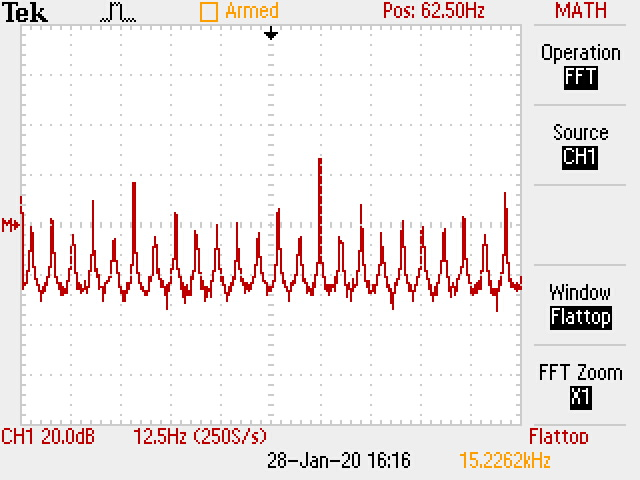
\includegraphics[width=\linewidth]{F0002TEK.JPG}
    \caption{Middle}
  \end{subfigure}
  \begin{subfigure}[b]{0.3\linewidth}
    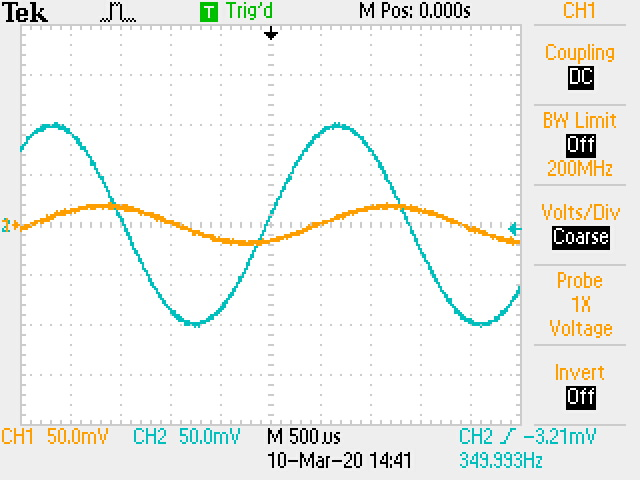
\includegraphics[width=\linewidth]{F0003TEK.JPG}
    \caption{Closer}
  \end{subfigure}
  \begin{subfigure}[b]{0.3\linewidth}
    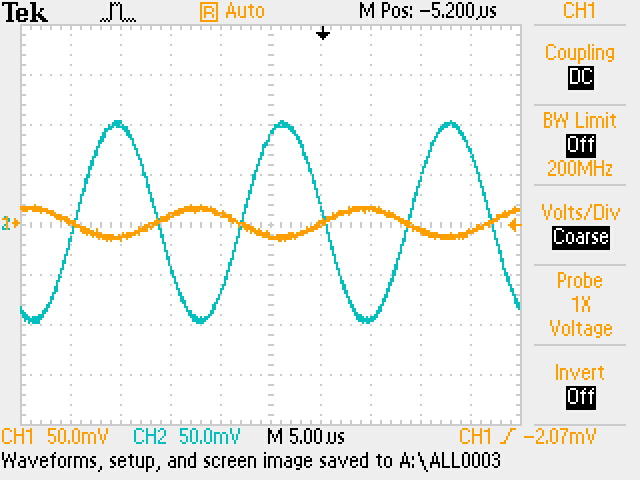
\includegraphics[width=\linewidth]{F0004TEK.JPG}
    \caption{Further}
  \end{subfigure}
  \caption{Фур'є перетворення}
\end{figure}
\clearpage
\subsubsection{Побудова фігур Лісажу}
\par\quadФігури Ліссажу - траєкторії, які прокреслюються точкою, що здійснює одночасно два гармонійних коливання у двох взаємно перпендикулярних напрямках.На практиці фігури Ліссажу можна отримати за допомогою осцилографа, якщо подати на нього два синусоїдальних сигнали, та відобразити по різним осям.
В ході роботи на один із каналів осцилографа Tektronix TDS 1002B подавався сигнал постійної частоти 1 кГц, тоді як частота сигналу на іншому каналі змінювалась від 0.5 до 2 кГц. Були отримані такі фігури(див Рис. 2, Рис. 3) 
\par\quad\begin{figure}[h!]
  \centering
  \begin{subfigure}[b]{0.4\linewidth}
    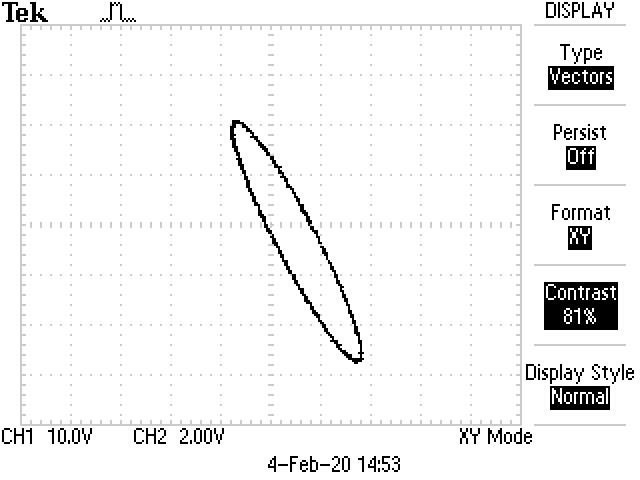
\includegraphics[width=\linewidth]{TEK0002.JPG}

  \end{subfigure}
  \begin{subfigure}[b]{0.4\linewidth}
    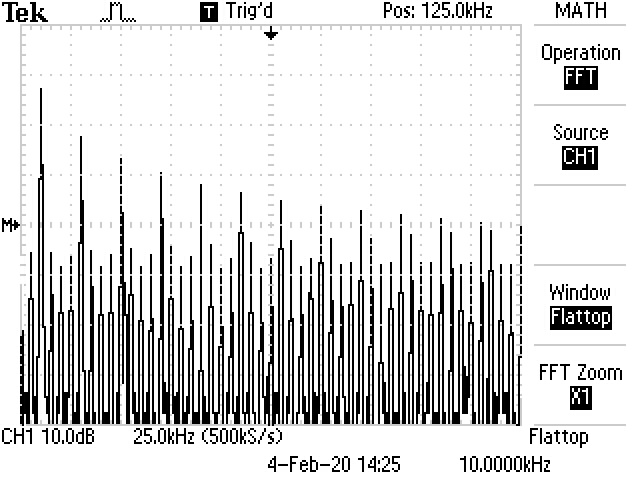
\includegraphics[width=\linewidth]{TEK0003.JPG}

  \end{subfigure}
  \begin{subfigure}[b]{0.4\linewidth}
    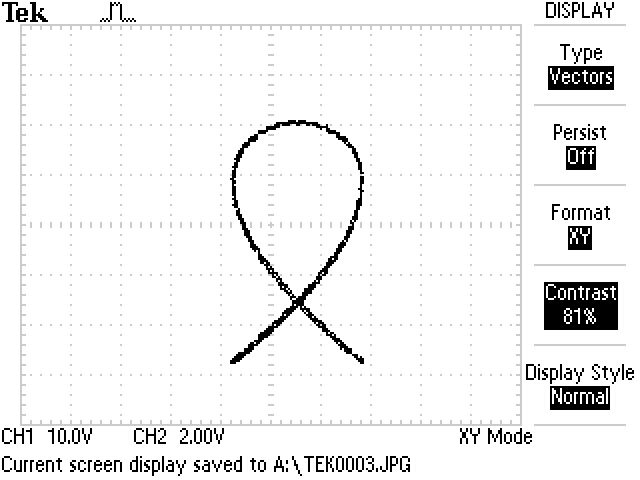
\includegraphics[width=\linewidth]{TEK0004.JPG}

  \end{subfigure}
  \begin{subfigure}[b]{0.4\linewidth}
    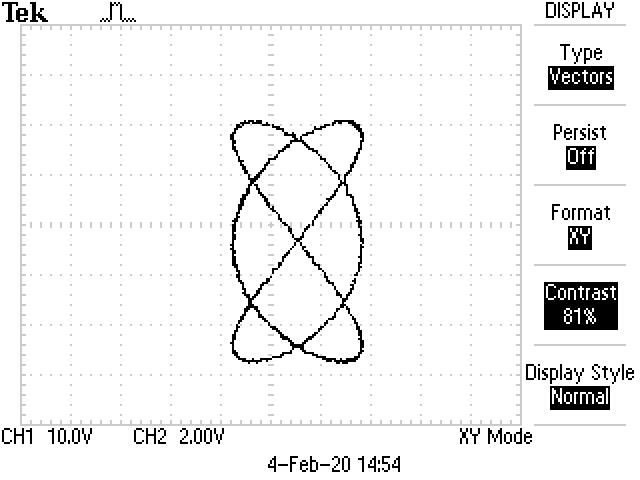
\includegraphics[width=\linewidth]{TEK0005.JPG}

  \end{subfigure}
    \caption{Фігури Лізажу}
\end{figure}  
\par\quad\begin{figure}[h!]
 \centering
  \begin{subfigure}[b]{0.4\linewidth}
    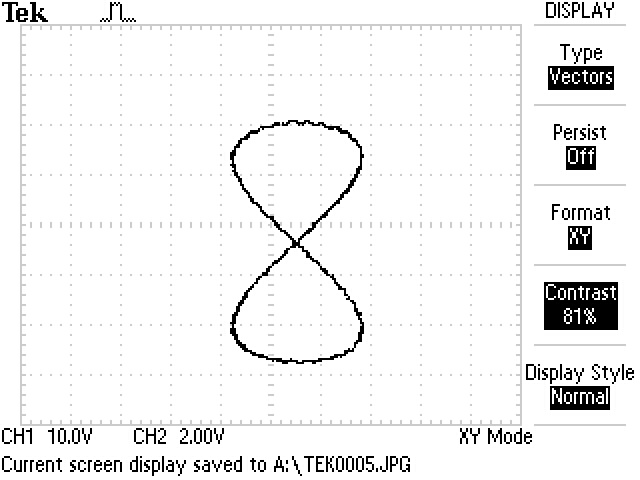
\includegraphics[width=\linewidth]{TEK0006.JPG}
    
  \end{subfigure}
  \begin{subfigure}[b]{0.4\linewidth}
    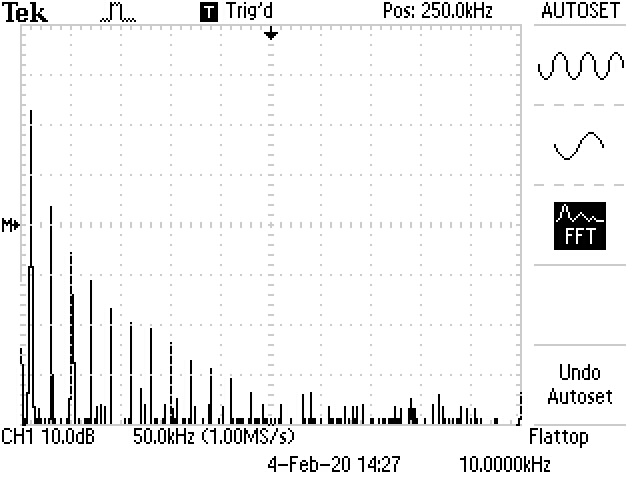
\includegraphics[width=\linewidth]{TEK0007.JPG}

  \end{subfigure}

 
  \begin{subfigure}[b]{0.4\linewidth}
    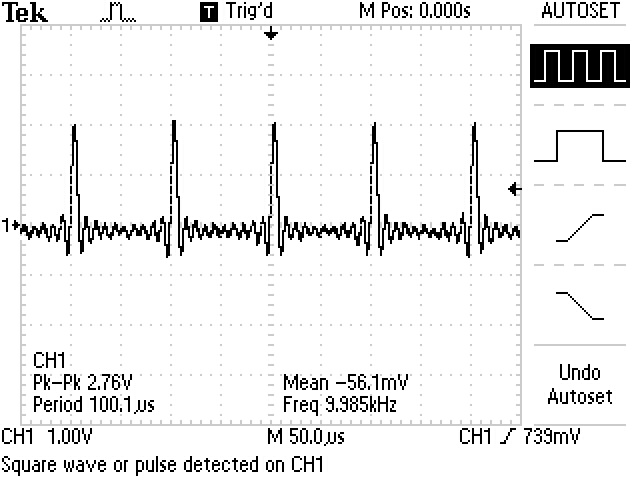
\includegraphics[width=\linewidth]{TEK0008.JPG}

  \end{subfigure}
  \begin{subfigure}[b]{0.4\linewidth}
    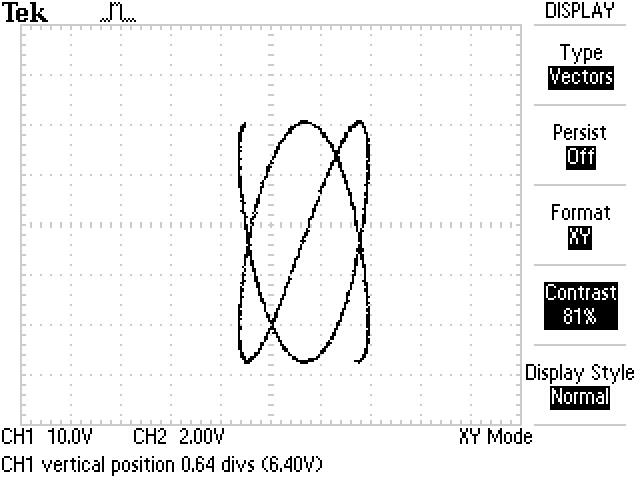
\includegraphics[width=\linewidth]{TEK0009.JPG}

  \end{subfigure}
  \caption{Фігури Лізажу}
\end{figure}

\clearpage\section{Висновки}
\par\quadУ результаті даної лабораторної роботи були проведені наступні вимірювання:
\par\quad1)На вимірювачі імпедансу HP 4192a:
\parОпір двох резисторів в залежності від частоти струму
\parЄмність та активний опір двох конденсаторів в залежності від частоти струму
\parІндуктивність та активний опір котушки в залежності від частоти струму
\par\quad2) На осцилографі Tektronix TDS 1002B:
\parБуло отримане перетворення Фур’є прямокутного сигналу.
\parБули отримані фігури Ліссажу для різних частот.
\end{document}